\documentclass{article}
\usepackage{graphicx} % Required for inserting images
\usepackage[utf8]{inputenc}
\usepackage{amsfonts}
\usepackage{amsmath}
\usepackage{amssymb}
\usepackage{amsthm}
\usepackage{float}
\usepackage{units}
\usepackage{wasysym}
\usepackage{mathabx}
\usepackage{subcaption}
\usepackage[margin= 0.5 in]{geometry}
\usepackage{hyperref}
\usepackage{authblk}
\usepackage{listings}
\usepackage{xcolor, colortbl}
\usepackage{wrapfig,lipsum,booktabs}

\usepackage{minted}
\usepackage{xcolor} 
\definecolor{LightGray}{gray}{0.9}
\definecolor{LightCyan}{rgb}{0.88,1,1}

\lstset{language=python,keywordstyle={\bfseries \color{blue}}}
\NewDocumentCommand{\codeword}{v}{%
\texttt{\textcolor{blue}{#1}}%
}

\setlength{\parskip}{1em}
\setlength{\parindent}{0em}

\title{CSC311 Project Report}
\author{Aryamann Rao, Paridhi Goel}
\date{28 March 2023}

\begin{document}

\maketitle

\section*{Part A}
\subsection*{k-Nearest Neighbour}
\subsubsection*{a)}
Given below in Figure \ref{fig:knn} a) is a plot of the accuracy of the user based collaborative filtering kNN model on the validation data set.

\begin{figure}[H]
    \centering
    \subfloat[User based collaborative filtering]{{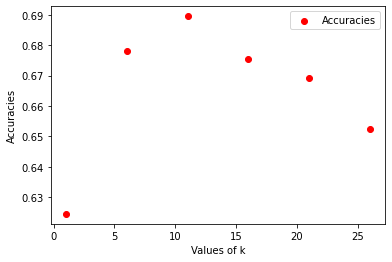
\includegraphics[width=8.5cm]{knn user accuracy.png} }}
    \qquad
    \subfloat[Item based collaborative filtering]{{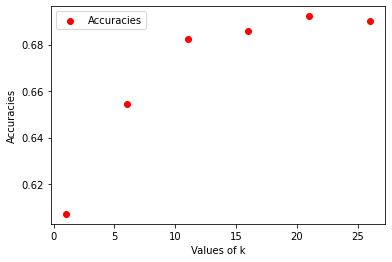
\includegraphics[width=8.5cm]{knn item accuracy.png}}}
    \caption{\textit{Left:} A plot of the validation accuracy of the user based collaborative filtering kNN model. \textit{Right:} A plot of the validation accuracy of the item based collaborative filtering kNN model.}
    \label{fig:knn}
\end{figure}

\subsubsection*{b)}
Here we observe the highest validation accuracy of $68.9\%$ at $k^*=11$. The test accuracy at this value of $k^*$ is $68.4\%$. 

\subsubsection*{c)}
Given in Figure \ref{fig:knn} b) is a plot of the accuracy of the item based collaborative filtering kNN model on the validation data set. Here we observe the highest validation accuracy of $69.2\%$ at $k^*=21$. The test accuracy at this value of $k^*$ is $68.2\%$. Item-based collaborative filtering approach relies on the assumption that questions that are hard for one student is also hard for another student i.e. similar questions are answered similarly by the students. This is possible if the "closeness" of two questions in data corresponds to them being of similar difficult and testing the similar content. 

\subsubsection*{d)}
We see that the test performance for user based collaborative filtering is $68.4\%$ at $k^*=11$ at which we receive the highest validation accuracy. However for item based collaborative filtering we get the highest validation accuracy at $k^*=21$ and the test accuracy at this value of $k^*$ is slightly lower than for user based collaborative filtering at $68.2\%$.

\subsubsection*{e)}
Limitations of kNN for the given task:
\begin{itemize}
  
  \item \textbf{User based collaborative filtering:} Here we predict the correctness based on the closest user. However, two students have different learning style, speed, and topic preferences. For example, it is possible that  two students, A and B, performed very similarly on trigonometry, but this does not mean they will perform similarly on number theory, a more unrelated field. It is possible that student A studied more number theory and performs significantly better on it. Similar performance in one area does not translate to similar performance in other areas. If the training data only includes diagnostic questions about specific topics in math, the performance of the model will be poor when we ask for predictions on questions about other topics.
  \item \textbf{Item-based collaborative filtering:} This approach relies on the assumption that questions that are hard for one student is also hard for another student. This does not account for the fact that student's ability are not equally distributed among topics. Some students are better at certain topics while others are not. If a student is particularly weak in a certain topic, we predict that the chances of a similar question being answered incorrectly are high, but this may not be true for all students. 
  \item Therefore, the major limitation in both these approaches is that kNN does not account for idiosyncrasies in the students' understanding of different topics. 
  \item Another limitation is that if a diagnostic question in the training set was not answered by many students, we many be unable to make reliable predictions i.e. we need to make sure all or at least most of questions in the training set are answered by many students to make accurate predictions.
  \item kNN model will not scale well if we add more students or questions because of high computational cost (need to store all of the training data in memory). 
\end{itemize}



\subsection*{Item Response Theory}
\subsubsection*{a)}
We know that the probability of the student $i$ answering the question $j$ correctly is given by,

$$p(c_{ij}=1|\theta_i, \beta_j)=\dfrac{e^{\theta_i-\beta_j}}{1+e^{\theta_i- \beta_j}}= \dfrac{1}{1+e^{-(\theta_i- \beta_j)}}=\sigma(\theta_i- \beta_j)=\sigma(z)$$

where we denote $z= \theta_i- \beta_j$. Similarly the probability of the student $i$ answering the question $j$ wrong is given by,

$$p(c_{ij}=0|\theta_i, \beta_j)=1-\dfrac{e^{\theta_i-\beta_j}}{1+e^{\theta_i- \beta_j}}=1-\sigma(z)$$

Thus we see that the logarithm of the probability can be written as,

$$\log[p(c_{ij}=1|\theta_i, \beta_j)]=
\begin{cases}
\log[\sigma(z)] &\text{if}\ c_{ij}=1\\
\log[1-\sigma(z)] &\text{if}\ c_{ij}=0\\
\end{cases}$$

Therefore the total negative log likelihood is expressed as,

$$\mathcal{L}= -\sum_{i,j}\log[p(c_{ij}=1|\theta_i, \beta_j)]$$

Taking the partial of the negative log likelihood with respect to $\theta_i$ is given by,

$$\dfrac{\partial \mathcal{L}}{\partial \theta_k}= -\sum_{i,j}\dfrac{\partial}{\partial \theta_k}\Big(\log[p(c_{ij}=1|\theta_i, \beta_j)]\Big)$$

where we have the relations for $\theta_i=\theta_k$ as shown below. If $\theta_i\neq \theta_k$ then the derivative is zero.

$$\dfrac{\partial}{\partial \theta_k}\Big(\log[p(c_{kj}=1|\theta_k, \beta_j)]\Big)=
\begin{cases}
\dfrac{\sigma'(z)}{\sigma(z)}\dfrac{\partial z}{\partial \theta_k} &\text{if}\ c_{kj}=1\\
\\
\dfrac{-\sigma'(z)}{1-\sigma(z)}\dfrac{\partial z}{\partial \theta_k} &\text{if}\ c_{kj}=0\\
\end{cases}$$

$$\implies \dfrac{\partial}{\partial \theta_k}\Big(\log[p(c_{kj}=1|\theta_k, \beta_j)]\Big)=
\begin{cases}
1-\sigma(z) &\text{if}\ c_{kj}=1\\
\\
-\sigma(z) &\text{if}\ c_{kj}=0\\
\end{cases}$$

Here we have used the relation $\sigma'(z)=\sigma(z)[1-\sigma(z)]$ and $\dfrac{\partial z}{\partial \theta_k}=1$. similarly taking the partial of the negative log likelihood with respect to $\beta_l$ is given by,

$$\dfrac{\partial \mathcal{L}}{\partial \beta_l}= -\sum_{i,j}\dfrac{\partial}{\partial \beta_l}\Big(\log[p(c_{ij}=1|\theta_i, \beta_j)]\Big)$$

where we have the relations for $\beta_j=\beta_l$ as shown below. If $\beta_j\neq \beta_l$ then the derivative is zero.

$$\dfrac{\partial}{\partial \beta_l}\Big(\log[p(c_{il}=1|\theta_i, \beta_l)]\Big)=
\begin{cases}
\dfrac{\sigma'(z)}{\sigma(z)}\dfrac{\partial z}{\partial \beta_l} &\text{if}\ c_{il}=1\\
\\
\dfrac{-\sigma'(z)}{1-\sigma(z)}\dfrac{\partial z}{\partial \beta_l} &\text{if}\ c_{il}=0\\
\end{cases}$$

$$\implies \dfrac{\partial}{\partial \beta_l}\Big(\log[p(c_{il}=1|\theta_i, \beta_l)]\Big)=
\begin{cases}
-[1-\sigma(z)] &\text{if}\ c_{il}=1\\
\\
\sigma(z) &\text{if}\ c_{il}=0\\
\end{cases}$$

Here we have used the relation $\dfrac{\partial z}{\partial \beta_l}=-1$. Therefore we derived the derivative of the negative log likelihood with respect to the parameters $\theta_k, \beta_l$ given by the equations above.

\subsubsection*{b)}
With a chosen hyperparameters of learning rate $0.01$ and $10$ iterations we obtain the negative log likelihood for the training and validation sets as shown in Figure \ref{fig:nnlk}.

\begin{figure}[H]
    \centering
    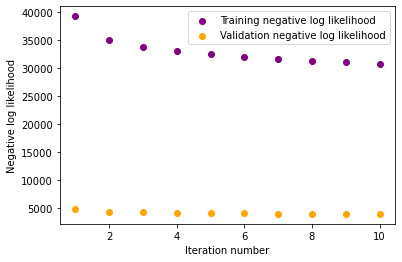
\includegraphics[width=9cm]{nnlk item response.png}
    \caption{Negative log likelihood for the training and validation sets variation with iteration.}
    \label{fig:nnlk}
\end{figure}

\subsubsection*{c)}
The final validation and testing accuracies after training are observed to be $70.69\%$ and $70.17\%$ respectively.

\subsubsection*{d)}
Consider the questions $j_1=10, j_2=20, j_3=30$ and suppose $\beta_{10}, \beta_{20}, \beta_{30}$ be the difficulties of the question. Now the variation of the probability that a student $i$ will answer each question correctly with their ability $\theta_i$ would be written as,

$$p_{10}=\sigma(\theta_i- \beta_{10})\ \text{and}\ p_{20}=\sigma(\theta_i- \beta_{20})\ \text{and}\ p_{30}=\sigma(\theta_i- \beta_{30})$$

Plotting these curves we see the result shown in Figure \ref{fig:questions},

\begin{figure}[H]
    \centering
    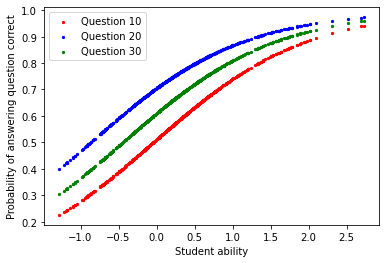
\includegraphics[width=9cm]{question answer item response.png}
    \caption{Variation of the probability that a student $i$ will answer each question correctly with their ability $\theta_i$.}
    \label{fig:questions}
\end{figure}

These curves have a shape very similar to that of the sigmoid function. This is expected as the probability function is a sigmoid function of the variable $z=\theta_i-\beta_j$. In our case we keep $\beta_j$ constant and change $\theta_i$. Physically these curves make sense as they represent the probability that a student with a given ability will answer the question correctly. Students with higher abilities have a higher change of answering the question correctly as per the graph which makes sense. Furthermore the more easier the question (represented by $\beta_j$) the higher it will be as students are more likely to answer it right.

\newpage
\subsection*{Neural Networks}
\subsubsection*{a)}
Three difference between ALS and neural networks:
\begin{itemize}
  \item ALS is a specific algorithm that solves the matrix completion problem and is usually used to implement collaborative filtering. Neural Networks are more general function approximators and can be used for variety of problems, including matrix completion (as a recommendation system), classification, image generation etc.  
  \item Unlike neural network, ALS minimizes two loss functions alternatively. Neural network only minimizes one function at each step. 
  \item Neural Networks (non linear deep auto encoders) can project the data onto a non linear manifold to achieve a non linear dimensionality reduction whereas ALS is a linear algorithm although we extend it using regularization. 
\end{itemize}
\subsubsection*{b)}
Completed in the \codeword{code.zip} file.

\subsubsection*{c)}
Figure \ref{fig:different k} shows a plot of the validation accuracy in the first epoch of the autoencoder neural net for various values of the latent dimension $k$ at a learning rate of $0.1$ and $\lambda=0$.

\begin{figure}[H]
    \centering
    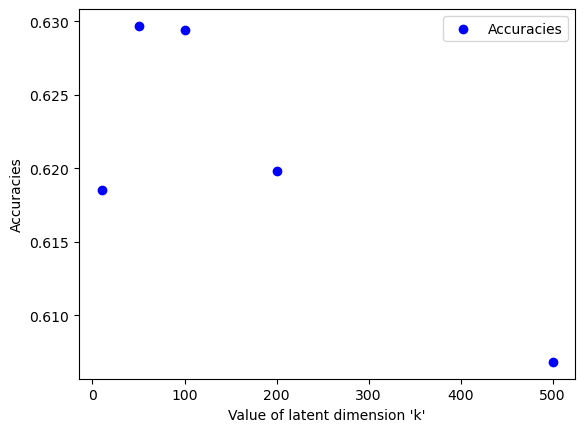
\includegraphics[width=8cm]{neural net original accuracy.png}
    \caption{A plot of the autoencoder accuracy for various values of $k$ at learning rate $0.1$ and $\lambda=0$.}
    \label{fig:different k}
\end{figure}

Here we see that $k^*=50$ reports the highest validation accuracy at the chosen hyperparameters. We will be using this value of $k^*$ for subsequent answers.

\subsubsection*{d)}
At $k^*=50$ we have plotted the training cost and the validation accuracy as a function of epoch for $10$ epochs in Figure \ref{fig:objectives}. Here we set the learning rate as $0.1$ and $\lambda=0$. The final test accuracy here was observed to be $66.6\%$.

\begin{figure}[H]
    \centering
    \subfloat[Training cost]{{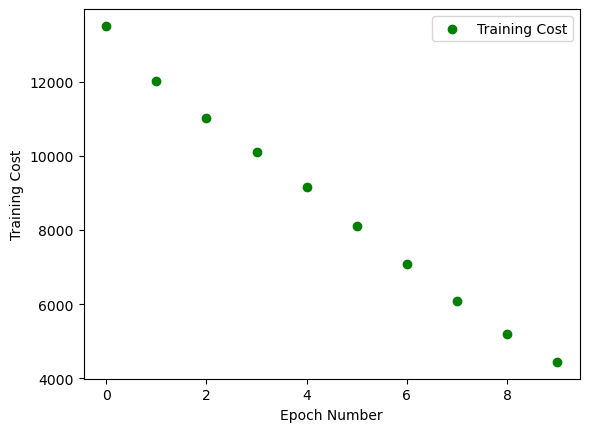
\includegraphics[width=7.5cm]{training objective.png} }}
    \qquad
    \subfloat[Validation accuracy]{{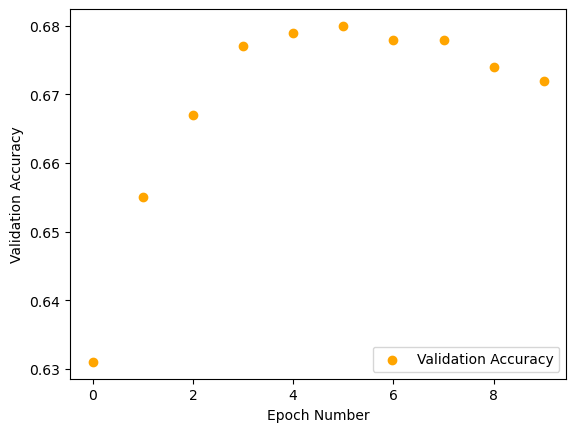
\includegraphics[width=7.5cm]{validation objective.png}}}
    \caption{\textit{Left:} Variation of the training cost as a function of epoch. \textit{Right:} Variation of the validation accuracy as a function of epoch.}
    \label{fig:objectives}
\end{figure}

\subsubsection*{e)}
Choosing the regularisation penalty from $\lambda\in \{0.001, 0.01, 0.1, 1.0\}$ we found that $\lambda = 0.01$ provided the highest testing accuracy of $66.9\%$ among all regularisation penalty values. Furthermore the validation accuracy increased in each epoch for all $10$ epochs which shows that the model was not overfitting since small changes in the weights was not decreasing the validation accuracies. Thus we will be using $\lambda=0.01$ for subsequent questions. Here the testing accuracy was slightly higher than without regularisation and hence we can say that the model performs slightly better with a regularisation term.

\subsection*{Ensemble}
We implemented a bagging ensemble to improve the stability and accuracy of our base models. We used 3 neural networks as our base models for the bagging. The final validation accuracy after 10 epochs was $67.1\%$ i.e. the ensemble model performed better than individual base models. The test accuracy for the ensemble model was $67.2\%$. 

For the ensemble process, we bootstrapped the given training set to sample data for the three base models. The base models (neutral networks) work with training data in the form a sparse matrix. Therefore, to sample data from the sparse matrix, we randomly set $12\%$ of the values in the given Sparse Matrix to NaN. We chose $12\%$ as it strikes a good balance between not removing too much data while sampling and also removing enough data to create some variability in the results of the base models that we later average out. We sample three training matrices from the original sparse matrix using this method and train the 3 models. Then we take the average of the prediction of the 3 models to get the combined prediction for the ensemble. We use this combined average prediction of find the training loss for the ensemble model.

We obtain better performance using the ensemble since it utilizes the "wisdom of crowds" which reduces variance and helps avoid overfitting. When multiple base models are aggregated, they can form a strong learner, as their combination reduces bias or variance, yielding better model performance. Since we select our initial weights randomly, each base model's performance varies slightly even on the same training data due to this randomness. Using, an ensemble stabilizes this variability too. 

\section*{Part B}
Autoencoders are a type of neural networks that learn by compressing the training data to a lower dimension to look for patterns in the data. They consist of an encoding part which compresses the input and a decoding part which decompresses the data to reconstruct the input. The goal of the model is to adjust the weights and biases of the neural connections such that the reconstruction of the input closely matches the original input. The loss function for a given set of weights $\bold{W}^{(1)}$ and $\bold{W}^{(2)}$ is given by the equation,

\begin{equation}
    \mathcal{L}= \sum_{v\ \in\ \mathcal{S}}||\bold{v}-f(\bold{v})||_2^2 + \dfrac{\lambda}{2}(||\bold{W}^{(1)}||^2+ ||\bold{W}^{(2)}||^2)
    \label{eqn:loss}
\end{equation}

where $f(\bold{v})$ is the reconstruction of the input and $\lambda$ is a hyperparameter that controls the regularisation component of the loss. The goal of this project is to minimise this loss and increase the accuracy of our model. 

\subsection*{The Base Model}
The base model we worked with was an Autoencoder with 3 layers. The middle layer had a length of $k$ which is our latent dimension while the input and output layers had a length of $N_{\text{questions}}$. Since the Autoencoders work by compressing the input, it means $k< N_{\text{questions}}$. The function $f$ that reconstructs the input can be written as,

\begin{equation}
    f(\bold{v})= \sigma(\bold{W}^{(2)}\sigma(\bold{W}^{(1)}\bold{v}+\bold{b}^{(1)})+\bold{b}^{(2)})
    \label{eqn:reconstruction}
\end{equation}

where $\sigma$ is the sigmoid activation function. Here the sigmoid function $\sigma(\bold{W}^{(1)}\bold{v}+\bold{b}^{(1)})$ represents the compression of the input to a lower dimensional subspace whose dimensionality is determined by the hyperparameter $k$. Furthermore the sigmoid function $\sigma(\bold{W}^{(2)}\sigma(\bold{W}^{(1)}\bold{v}+\bold{b}^{(1)})+\bold{b}^{(2)})$ represents the decompression of the compressed input to reconstruct it back to its original dimensionality. Figure \ref{fig:autoencoder} below depicts a visual representation of our base model.

\begin{figure}[H]
    \centering
    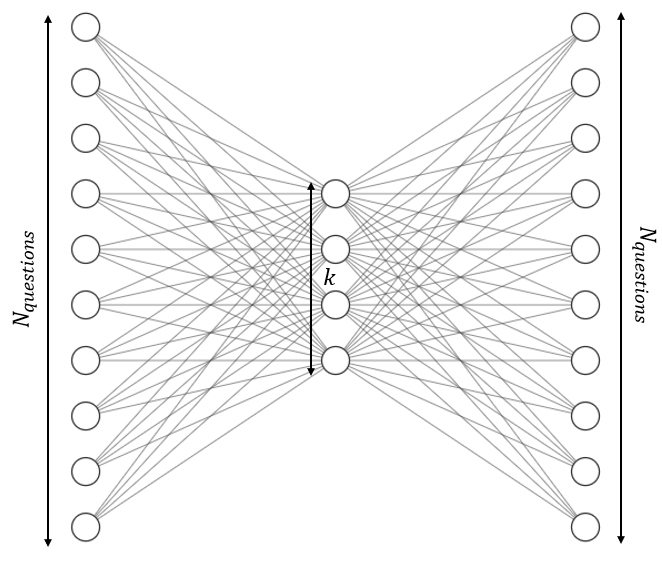
\includegraphics[width=6.5cm]{autoencoder.png}
    \caption{A diagram showing a visual representation of the base model of our autoencoder. Please note that the number of nodes do not represent the true dimensions of our model. This is because $N_{\text{questions}}=1774$ which is difficult to depict.}
    \label{fig:autoencoder}
\end{figure}

\subsection*{Extending the Model}
The base model we initially worked with had some limitations and did not have a very good accuracy. More specifically our model was underfitting the data as the validation accuracy and the test accuracy were around $66\%$ which means the model was unable to find many patterns in the data. To fix this problem we made two major extensions to our base model:

\begin{enumerate}
    \item Added more layers to the neural network.
    \item Extended the input vector to include more features about the student such as their age, gender and economic situation.
\end{enumerate}

Although the first extension resulted in an improved accuracy in the later epochs, the second extension reduced the accuracy and the reason for this has been explored. We have submitted two files \codeword{neural_network_modified_1.py} and \codeword{neural_network_modified_2.py}. The former with the first extension only and the latter with both extensions applied. The following subsections go into detail into the processes involved in implementing these extensions.

\subsubsection*{Extension 1: Adding Layers to the Network}
As mentioned before, autoencoders work by compressing and decompressing the input to create a reconstruction of it. This enables it to reduce any prevalent noise in the data which makes it easier to look for patterns. Theoritically, the more one compresses the input, the more the neural network will be able to find patterns. However at the same time we need to be careful to not compress the data too much which might lead to true information loss. Thus we introduced two new layers to our base model to improve optimisation of our model. Figure \ref{fig:modified autoencoder} below shows a schematic diagram of the extension described in this section.

\begin{figure}[H]
    \centering
    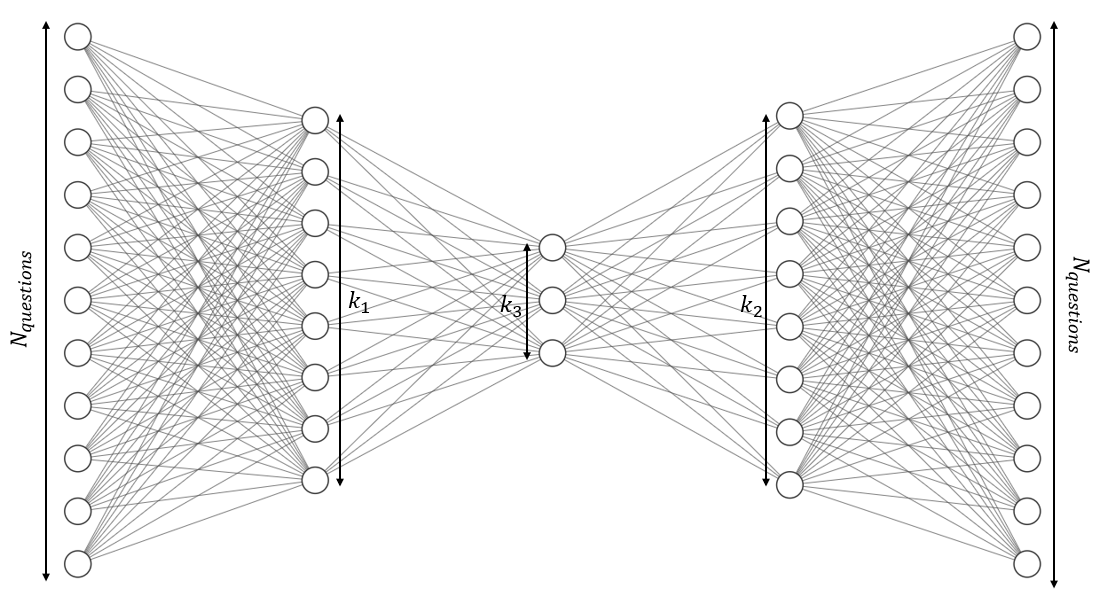
\includegraphics[width=10cm]{modified encoder.png}
    \caption{A diagram showing a visual representation of the base model of our modified autoencoder with the first modification. Please note that the number of nodes do not represent the true dimensions of our model. This is because $N_{\text{questions}}=1774$ which is difficult to depict.}
    \label{fig:modified autoencoder}
\end{figure}

As can be seen from Figure \ref{fig:modified autoencoder} this extension brings two new hyperparameters $k_1$ and $k_2$ that describe the model which are labelled above. To ensure compression of the data we had to impose the restriction that $k_2<k_1$. Mathematically the function that describes this model can be thought of as composition of four functions $f_1, f_2, f_3, f_4$ where $f_i$ is the function that takes the result from layer $i$ and transmits it to layer $i+1$. Thus we can express this as,

\begin{align}
    f_1(\bold{v}) &= \sigma(\bold{W}^{(1)}\bold{v}+\bold{b}^{(1)})\\
    f_2(\bold{v}) &= \sigma(\bold{W}^{(2)}f_1(\bold{v})+\bold{b}^{(2)})\\
    f_3(\bold{v}) &= \sigma(\bold{W}^{(3)}f_2(\bold{v})+\bold{b}^{(3)})\\
    f_4(\bold{v}) &= \sigma(\bold{W}^{(4)}f_3(\bold{v})+\bold{b}^{(4)})
    \label{eqn:modified neural net function}
\end{align}
    
where $\bold{W}^{(1)}, \bold{W}^{(2)}, \bold{W}^{(3)},\bold{W}^{(4)}$ and $\bold{b}^{(1)}, \bold{b}^{(2)}, \bold{b}^{(3)},\bold{b}^{(4)}$ are new sethttps://www.overleaf.com/project/642345b46d59eed564e2d4d0s of weights and biases corresponding to the extended neural network.  Evaluating each of these functions in the order mentioned above, we could construct the forward pass of our modified neural net. The values of the hyperparameters $k_1, k_2$ were tuned such that the information was sufficiently compressed but not excessively so to prevent the loss of actual patterns in the data. We observed the highest validation accuracy at $k_1= 50$ and $k_2=2$. The results have been plotted in Figure \ref{fig:extended models}. However this extension still did not take into consideration various features of the students that could potentially influence their answers to exam questions. We had information on their age, gender and economic situation. Therefore we attempted to extend the network to include these features in the learning stage.

\subsubsection*{Extension 2: Including Student Metadata}
To factor in various features that define a student we decided to include the information included in the \codeword{student_metadata.csv} file regarding the characteristics of various students. The student data in this file was sorted according to their user id and the relevant information such as age, gender and economic status were appended to the input vector $\bold{v}$. A new function \codeword{load_student_metadata()} in \codeword{utils.py} that loaded the metadata and appended it to our vector. Thus we now had a train matrix of dimensions $N_{\text{students}}\times (N_{\text{questions}}+3)$. This extension was added along with Extension 1 and the results have been plotted in Figure \ref{fig:extended models}. The purpose of adding this extension was to find patterns in the student's features that could influence their ability to answer the questions correctly.

\subsection*{Results}
Given in Figure \ref{fig:extended models} is a comparison of the validation accuracies per epoch of the base model and the model with extension 1 and 2 applied. It should be noted that due to a larger number of weights introduced in both extensions, the regularisation contributed a lot more to the loss than in the base model. Thus we had to set the regularisation parameter to $\lambda=0$ to achieve the results in Figure \ref{fig:extended models}. The learning rate however was kept constant as in the base model.

\begin{figure}[H]
    \centering
    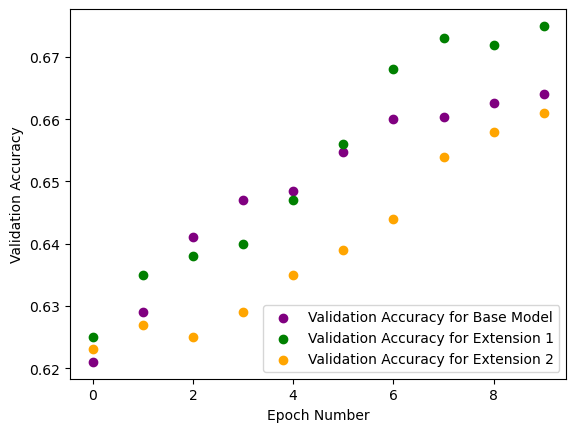
\includegraphics[width=9cm]{extended accuracy.png}
    \caption{A comparison of the validation accuracies of the neural nets model considering both extensions w.r.t epoch.}
    \label{fig:extended models}
\end{figure}

It should be noted that the accuracies noted above will not be the same every time the code is run. This is because the model initialises the weights randomly and thus every run has a different learning outcome which can change the accuracies. However on average the results were consistent with what has been outlined above. Here we see that although the model with extension 1 performed better than our base model in later epochs, applying extension 2 slightly reduced the validation accuracies. This could be because the values of the age of the students can be any real number and is not limited between $0$ and $1$. Furthermore males are represented by the integer $2$. Therefore the sigmoid functions used in Equation \ref{eqn:modified neural net function} could not accurately reconstruct the input as the output of these functions as a sigmoid only outputs values between $0$ and $1$. If we had more time, we would explore using different activation functions like ReLU to solve this problem.

\subsection*{Limitations}
It is expected that the accuracy of machine learning models improves with more data. Therefore, if we deploy this encoder-based model to determine patterns in a situation where sufficient data is not available it will perform poorly. 

A more specific limitation of the our model was the reduced validation accuracy after Extension 2. Usually, adding more data improves the prediction. However, we saw a decrease in the validation accuracy after adding the student metadata to the training matrix. In Extension 2, we extended our training matrix by adding data about the student's age, gender and economic background. However, this data cannot easily be represented by numbers 0 and 1, like all the other entries in the training matrix. This creates a problem because our neural network uses sigmoid function as its activation and cannot output numbers greater than 1. 

One possible way to overcome this limitation is to normalise the age data and gender data. For example, we could represent gender by using 0.5 for female, 1 for male and 0 for unspecified instead of the given values 1, 2, 0 respectively. We could not try this approach due to shortage of time. However, one can extend this project by working on normalising the metadata for the training. 

Another possible way to improve the performance of this model is to include the data about more students and questions. The data given to us for training was sub sampled from the dataset provided by Eedi, an online learning platform. The data consisted of answers of 524 students to 1773 diagnostic question. However, it is likely that using a bigger sub sample of Eedi's data will improve the accuracy because autoencoders, as an unsupervised algorithm, require a significant amount of clean data to generate useful results. 


\section*{Contributions by Team Members}
 
 
\begin{itemize}
  
  \item \textbf{Aryamann Rao:} kNN, Neural Networks for Part A
  \item \textbf{Paridhi Goel:} Ensemble for Part A
  \item Both members worked together on IRT from Part A and Part B
\end{itemize}
\end{document}
